
% http://patorjk.com/software/taag/#p=display&f=Colossal&t=ABOUT
\documentclass[runningheads,a4paper,oribibl]{llncs}
%\setcounter{secnumdepth}{4}

\usepackage[T1]{fontenc}

\usepackage[utf8]{inputenc}
% \usepackage[latin1]{inputenc}
\usepackage{textcomp}
\usepackage{graphicx}    
\usepackage{url}
\usepackage{pdfpages}          

\begin{document}

\pagestyle{headings}

\mainmatter

\title{Exploring the differences in performance between gamers and non-gamers when completing everyday tasks viewed from a third-person perspective}


\titlerunning{Third-Person Performance Differences Between Gamers and Nongamers}

\author{Arvid Bräne}

\institute{
	Department of Computing Science \\
	Umeå University, Sweden \\
	\email{arvidbrane@gmail.com} 
}

\maketitle


\begin{abstract}
	

The abstract will include the following:
\begin{itemize}
	\item What have I done?
	\item How did I do it?
	\item What was the result of the study?
	\item What to take out from this study.
	\item Results suggest ...
\end{itemize}

\end{abstract}









% 8888888 888b    888 88888888888 8888888b.   .d88888b.  
%   888   8888b   888     888     888   Y88b d88P" "Y88b 
%   888   88888b  888     888     888    888 888     888 
%   888   888Y88b 888     888     888   d88P 888     888 
%   888   888 Y88b888     888     8888888P"  888     888 
%   888   888  Y88888     888     888 T88b   888     888 
%   888   888   Y8888     888     888  T88b  Y88b. .d88P 
% 8888888 888    Y888     888     888   T88b  "Y88888P"  


\section{Introduction}
% Description of what third-person view is


There is a constantly ongoing debate of whether playing video games produce negative side-effects or not~\cite{tear2014video}. Some earlier findings indicate that committing ``immoral'' virtual behaviors in a video game can lead to increased moral sensitivity of the player~\cite{grizzard2014being}. Others studies point towards that playing video games do not have any effect on depression, hostility, or, visuospatial cognition~\cite{valadez2012just}. There are even results in experiments that suggest the opposite; violent games reduce depression and hostile feelings in players through mood management~\cite{ferguson2015hitman}. 

On the contrary, some research hint that video games can result in \emph{positive} side-effects such as improved cognitive control, emotional regulation, spatial resolution of vision, hand-eye motor coordination, and contrast sensitivity~\cite{gong2015enhanced}. Other results point towards an improved probabilistic inference without loss of measurable accuracy~\cite{green2010improved}.

Studies in literature have previously shown that most readers do not have any recognition about whether a book they have read was written in first- or third-person~\cite{hagg2012nya} due to humans capability of ``translating'' and adapting from one pronouns to another. Kohler's experiments with inverted vision goggles showed subjects walking and riding bicycles while seeing upside-down~\cite{kohler1962goggles}, pointing towards even greater capability of the human brains ability to adapt. This could suggest that users might be able to adapt to seeing themselves from third-person perspective.

This study aims to investigate if there is a measurable difference in performance, such as number of errors made and time consumption, between people who have played games and people who have not when they are prompted to complete everyday-like tasks viewed from third-person perspective (see Fig~\ref{fig:GTAIV}). Similar studies have been conducted, such as~\cite{schmierbach2011exploring} and~\cite{nakamura20103pi}, but certain aspects about performance differences in everyday tasks remain unaddressed. The study was completed using a custom-made rig in order to fully simulate the experience of a life viewed from a third-person perspective.













% 888b     d888 8888888888 88888888888 888    888  .d88888b.  8888888b.  
% 8888b   d8888 888            888     888    888 d88P" "Y88b 888  "Y88b 
% 88888b.d88888 888            888     888    888 888     888 888    888 
% 888Y88888P888 8888888        888     8888888888 888     888 888    888 
% 888 Y888P 888 888            888     888    888 888     888 888    888 
% 888  Y8P  888 888            888     888    888 888     888 888    888 
% 888   "   888 888            888     888    888 Y88b. .d88P 888  .d88P 
% 888       888 8888888888     888     888    888  "Y88888P"  8888888P"  

\section{Material \& Method}
Studies prior to this one have been done on the differences between gamers and non-gamers, such as~\cite{schmierbach2011exploring} and~\cite{gong2015enhanced}, but none using hardware to simulate the out-of-body, third-person view experienced in games (see Fig~\ref{fig:GTAIV}) in real life. Our method of choice was to construct a custom designed rig where subjects saw themselves, in real-time from a third-person perspective. In order to see the differences between gamers and non-gamers the test subjects had to complete the same three tasks, in three different configurations, three times in a row. After the subjects finished their participation, they were prompted to fill in a form regarding the experience and their prior experience with video games. The two groups, consisting of 13\footnote{14 subjects were originally in the study, but one male could not complete the whole experiment due to the his poor eyesight when not wearing his glasses. He was therefore excluded from the study after the first task and not included int the results.} subjects (undergraduate volunteers, high male skew\footnote{12 male subjects and 2 female, in ages ranging from 23 to 28}), were then benchmarked against each other to see which performed better. In the following subsections we will thoroughly demonstrate the different steps in our method and the tasks needed to later concretize credible results.









\begin{figure}
   \centering
   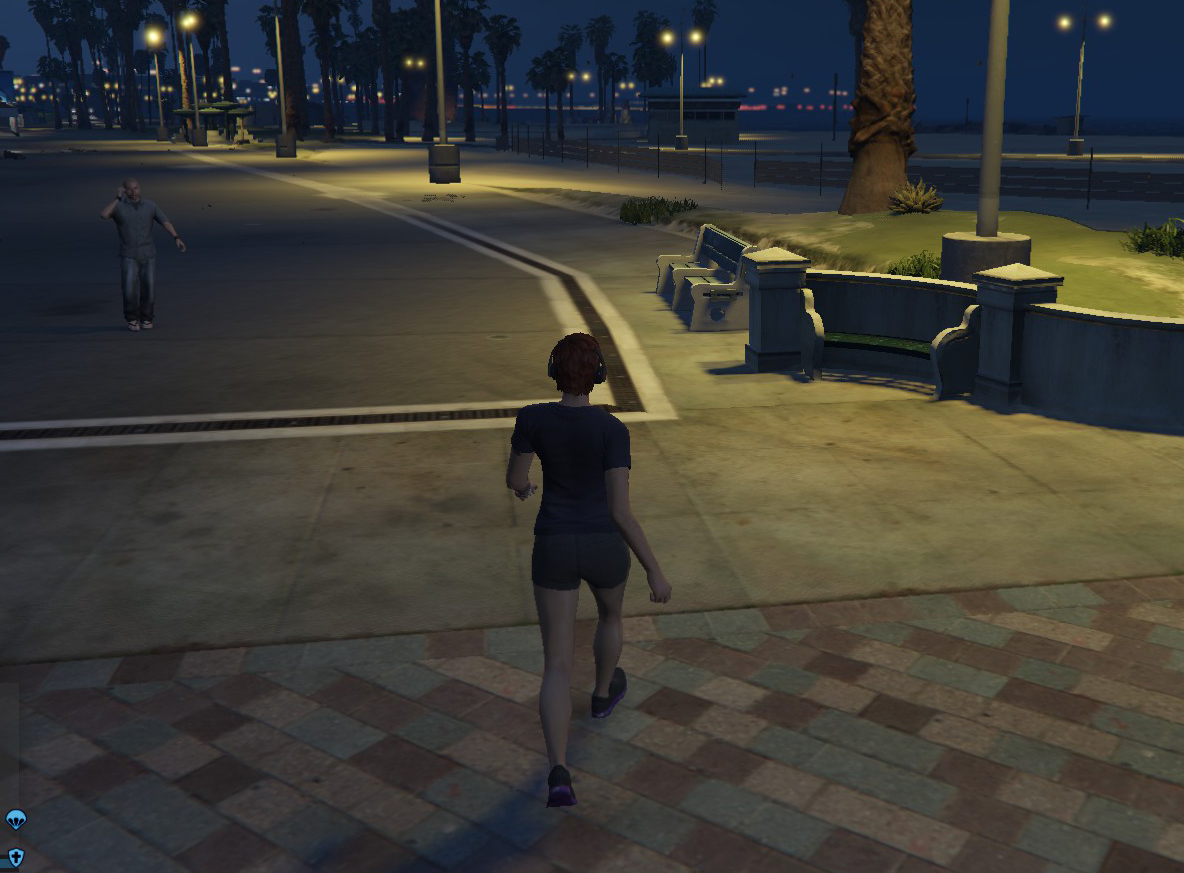
\includegraphics[width=\textwidth]{ExternalMaterial/GTA}
   \caption{A typical third-person perspective in a game from the game \emph{Grand Theft Auto: V}. \label{fig:GTAIV}}
\end{figure}









\subsection{Task Design} \label{subsec:TaskDesign}

In order to get the required measurements with high credibility the tasks performed by the test subjects were carefully planed, pilot-tested, prepared, executed and then evaluated. To get as general spread results as possible 3 different types of tasks had to be completed by each test subject.

\subsubsection{Task 1: Accuracy}

The test subjects rolled, threw or bounced (depending on their preference) a multi-colored volleyball in order to try and hit a target (a regular sized chair) placed approximately 5 meters away to successfully complete the task (see Fig~\ref{fig:AccuracyTask}). If the test subject missed the target they were told to try again until the finally hit the target. This test measured the participants precise accuracy and ball control through the number of tries required in order to hit the target.

\begin{figure}
   \centering
   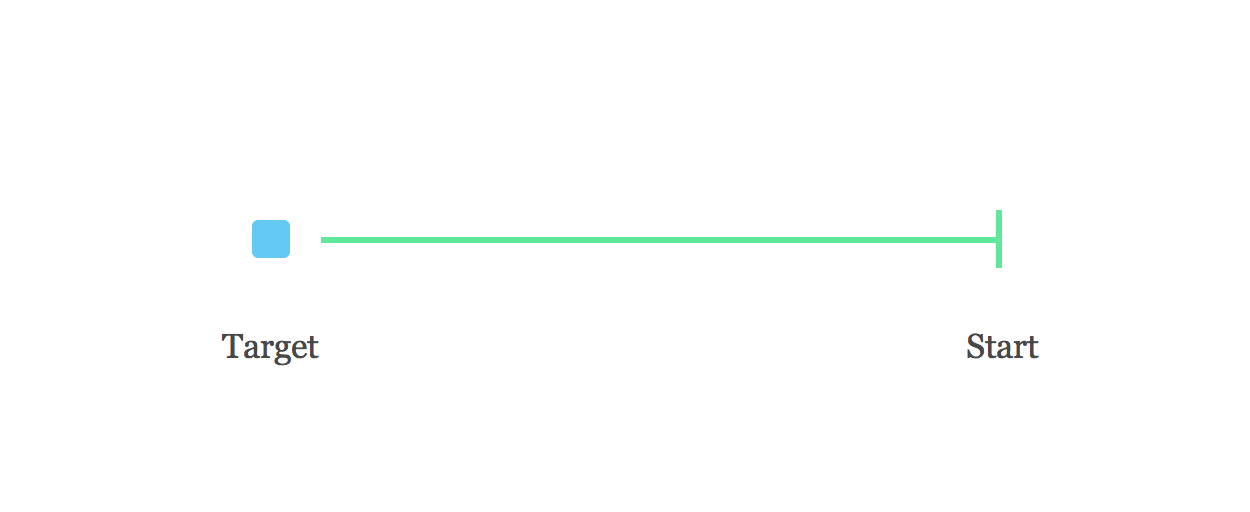
\includegraphics[width=0.7\textwidth]{ExternalMaterial/AccuracyTask}
   \caption{A \emph{side-view} of the course used during Accuracy Task where green is tape on the floor and blue is the chair.}. \label{fig:AccuracyTask}
\end{figure}

\subsubsection{Task 2: Balance}

The test subjects walked, in their preferred speed, on a thin straight line made out of tape, measured at 10 meters long (see Fig~\ref{fig:BalanceTask}), placed on the ground. This test measured the participants balance skills through the number of errors they made. These errors were objectively measured and recorded using one pre-defined rule; if any part of the shoe/foot covered the width of the tape (approximately 2 centimeters wide) it was considered to be a legal foot placement, everything else was illegal. An example of an illegal foot placement can be found in Fig~\ref{fig:Illegal} and a legal example can be found in Fig~\ref{fig:Legal}.

\begin{figure}
   \centering
   \includegraphics[width=0.6\textwidth]{ExternalMaterial/Legal}
   \caption{Two examples of \textbf{legal} foot placements.} \label{fig:Legal}
\end{figure}

\begin{figure}
   \centering
   \includegraphics[width=0.6\textwidth]{ExternalMaterial/Illegal}
   \caption{Two examples of \textbf{illegal} foot placements.} \label{fig:Illegal}
\end{figure}

\begin{figure}
   \centering
   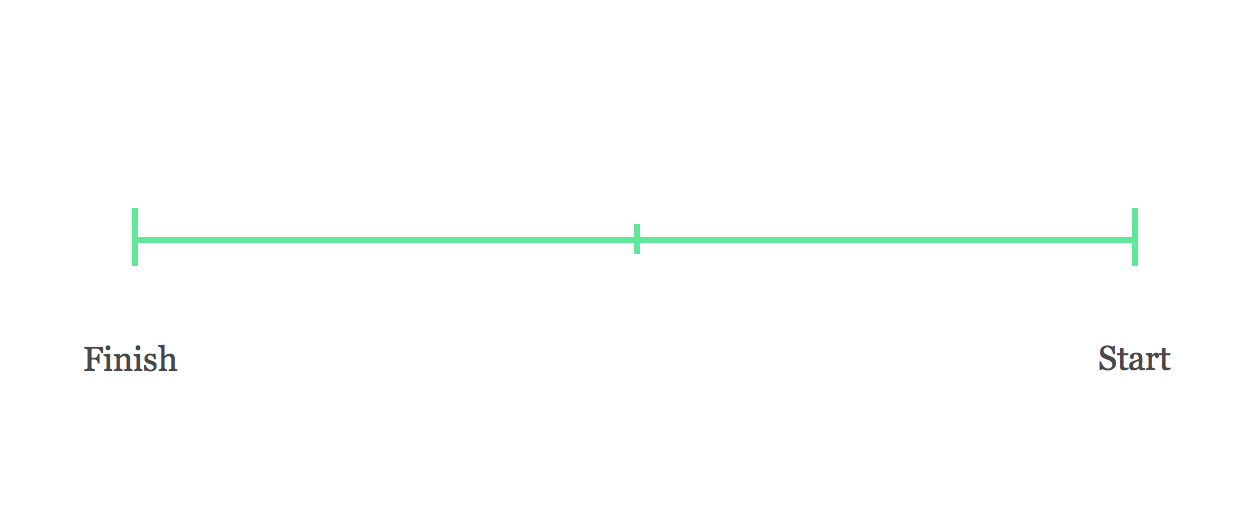
\includegraphics[width=0.7\textwidth]{ExternalMaterial/BalanceTask}
   \caption{An approximate \emph{top-view} of the curse used during the Balance Task where green is tape on the floor.} \label{fig:BalanceTask}
\end{figure}

\subsubsection{Task 3: Movement}

The test subjects walked, facing forward, in their normal walking speed, thorough a pre-planned course approximately 25 meters long and circa 2 meters wide (see Fig~\ref{fig:Course}) without touching anything other than the floor. The course was constructed using 40 chairs, 5 tables, 1 large wooden box, 5 meter long wall and a tall pillar(see Fig~\ref{fig:CourseTop}). Participants started between two chairs on the right and finished when they stepped on the cross marked with tape on the floor. This test measured the participants movement and navigational skills through the required time in order to complete the task. Errors made, such as touching the chairs or tables, were also recorded.

\begin{figure}
   \centering
   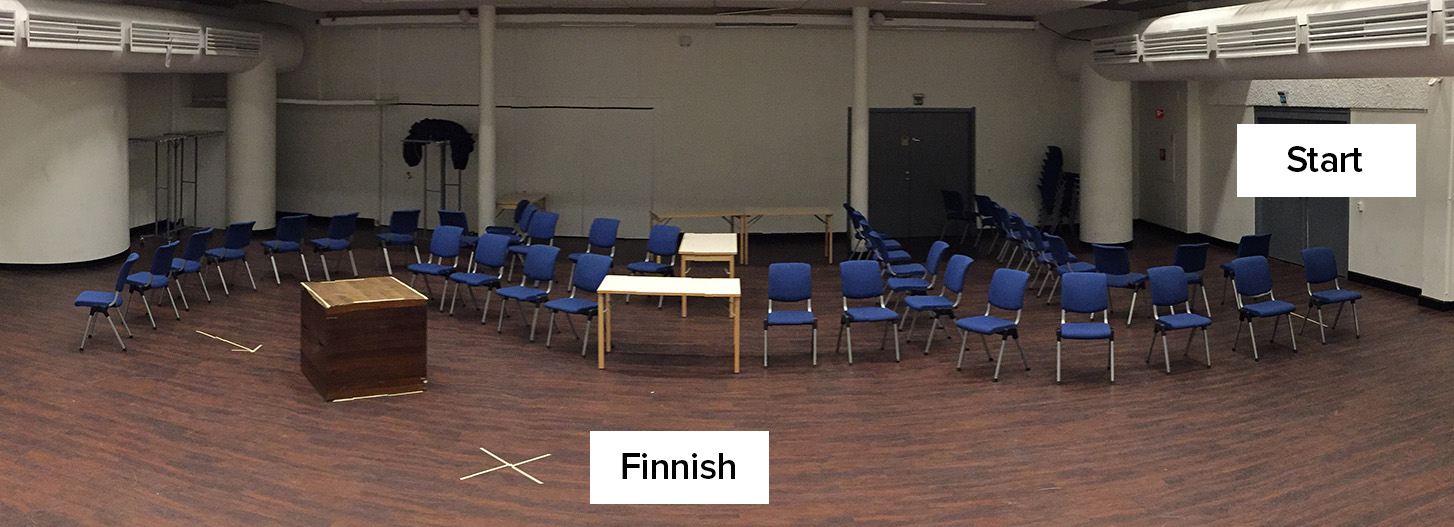
\includegraphics[width=\textwidth]{ExternalMaterial/Course2}
   \caption{A \emph{side-view} of the course used during the Movement Task.} \label{fig:Course}
\end{figure}

\begin{figure}
   \centering
   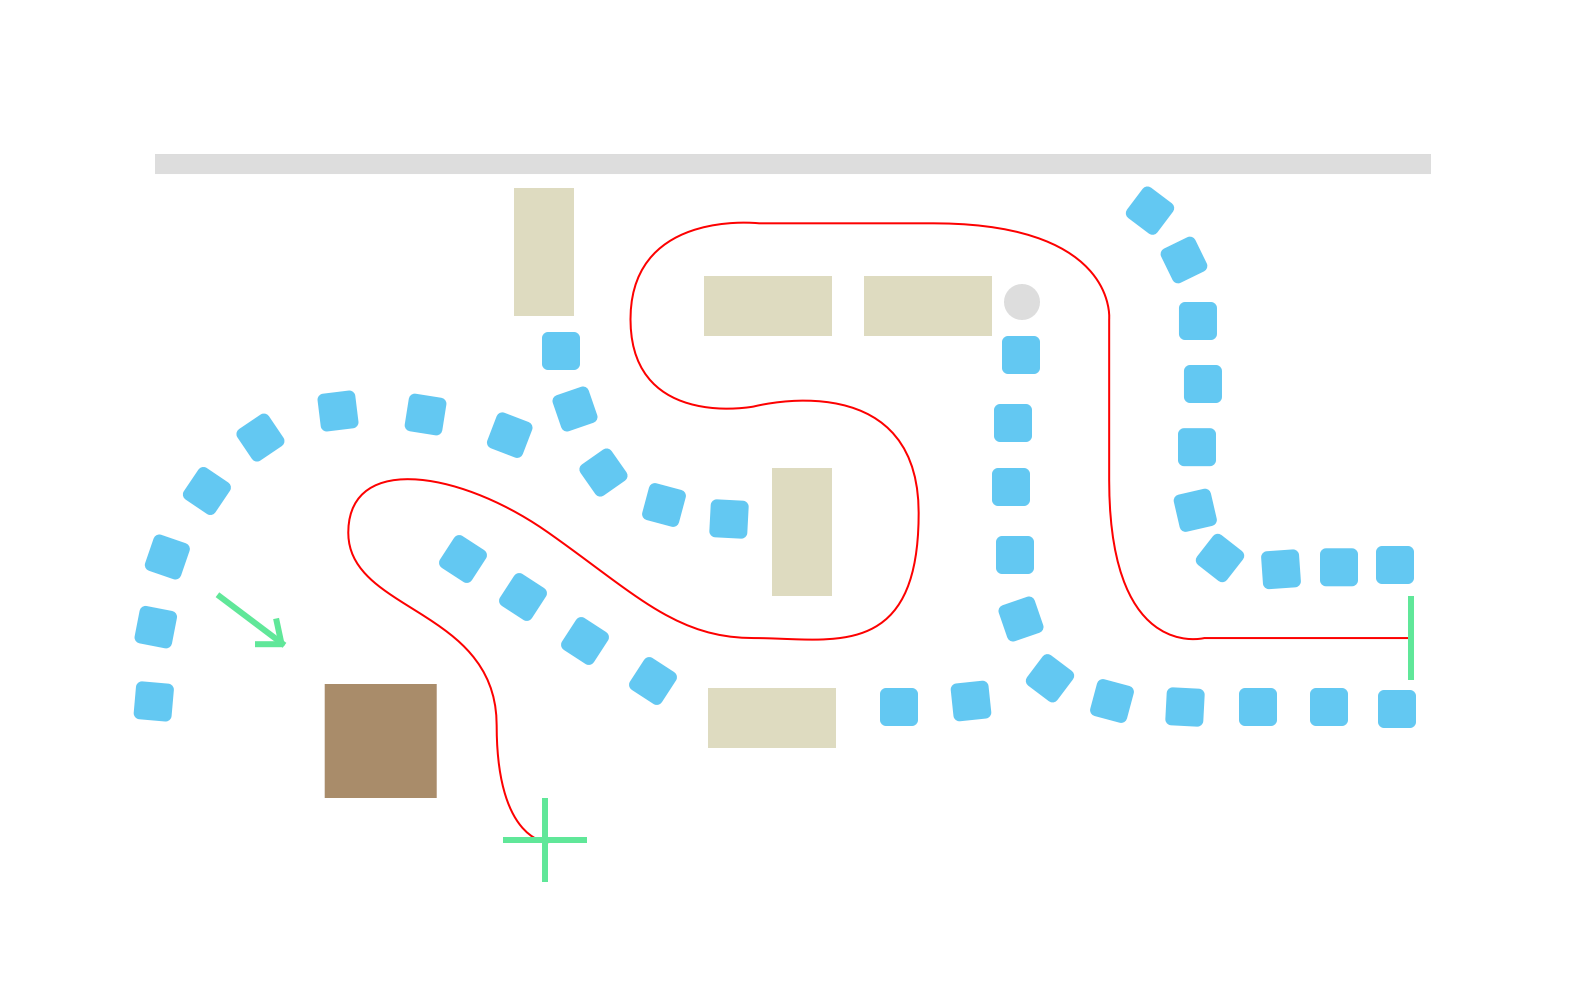
\includegraphics[width=\textwidth]{ExternalMaterial/Course-top}
   \caption{A \emph{top-view} of the course used during the Movement Task where red is the approximate distance where the participants walked, beige are tables, blue are chairs, green is tape on the floor, brown is the wooden box and gray is the wall and pillar.} \label{fig:CourseTop}
\end{figure}


\subsubsection{Configurations} \label{subsubsec:Configurations}
Each task was performed \emph{3 times} by each participant, in 3 different configurations resulting in a total of nine results for each participant. The different configurations were completed in the following order:
\begin{enumerate}
	\item \textbf{Off}: \emph{Not} wearing the rig, video goggles \emph{off}.
	\item \textbf{First-Person}: Wearing the rig, video goggles \emph{on}, viewed from \emph{first-person} camera.
	\item \textbf{Third-Person}: Wearing the rig, video goggles \emph{on}, viewed from \emph{third-person} camera.
\end{enumerate} 

Completing the task 3 times was done to get an accurate estimate of each of the participants performance. Completing the task in 3 different configurations was done to minimize the effects of individual differences amongst the test subjects. 

The first configuration served as a baseline for how a participant performs when completing the task ``normally''. The second configuration was used to compare against the first configuration in order to understand how much the video goggles and the first-person camera affected the participants performance in completing the tasks. Comparing the third configuration and the second configuration was the main focus of this study which was why the third configuration was the most critical one.










\subsection{Rig Design}
In order to simulate a game-like, out-of-body experience and a third-person perspective (see Fig~\ref{fig:GTAIV}), without leaving the participants nauseated\footnote{Early test showed that participants felt sea-sick due to unwanted camera movement created by an unstable test-rig.} the rig had to be as rigid as possible. The main parts in the rig were:
\begin{description}
	\item[Back \&\ Camera Mount] A solid mounting foundation was constructed out of light weight and stiff materials such as carbon fiber, ABS and polymorph plastic. As a base for the whole construction a snowboard back protector was used in order to connect the carbon fiber rods to the subjects back. Some 3D-printed parts where used to fasten the third-person camera to the subject.

	\item[Third-Person Video Camera] The video camera used for the third-person view, constantly generating a live video stream, was mounted on a pole circa a meter approximately 45 degrees above/behind the participants head and tilted circa 30 degrees downwards in order to frame the video correctly. Since a large field-of-view, a compact- and lightweight design are the most important requirements for selecting the video camera a \emph{GoPro Hero 3: Black Edition}\footnote{More info can be found at http://www.prisjakt.nu/produkt.php?e=1457108} was chosen, weighing 163 grams and a field-of-view at 170 degrees. The camera was connected to the participants video goggles using a 3 meter long, 4 pole and a cable.

	\item[Video Goggles \&\ First-Person Video Camera] To cover the subjects eyes and view the live video stream a pair of specially designed video goggles were used. These goggles, a pair of \emph{SkyZone SKY-01 V2}\footnote{More info can be found at http://www.foxtechfpv.com/skyzone-fpv-gogglesmatte-blackpreorder-p-1218.html}, have a field-of-view of approximately 30 degrees and a built in camera with a diagonal field-of-view at 120 degrees. This camera was used for the second configuration for each task (described in Section~\ref{subsubsec:Configurations}) to simulate first-person perspective.
\end{description}
The final result of the rigs design is somewhat inspired by~\cite{salamin2010quantifying} (but with more up-to-date hardware) and can be found in Fig~\ref{fig:RigDesign} along with what the user saw\footnote{The top and bottom of the image is cut of due to the camera not being able to capture non-wide screen video. During the experiment the user was able to see approximately 30 centimeters behind his/hers feet.} in Fig~\ref{fig:3Pview}.





\begin{figure}
   \centering
   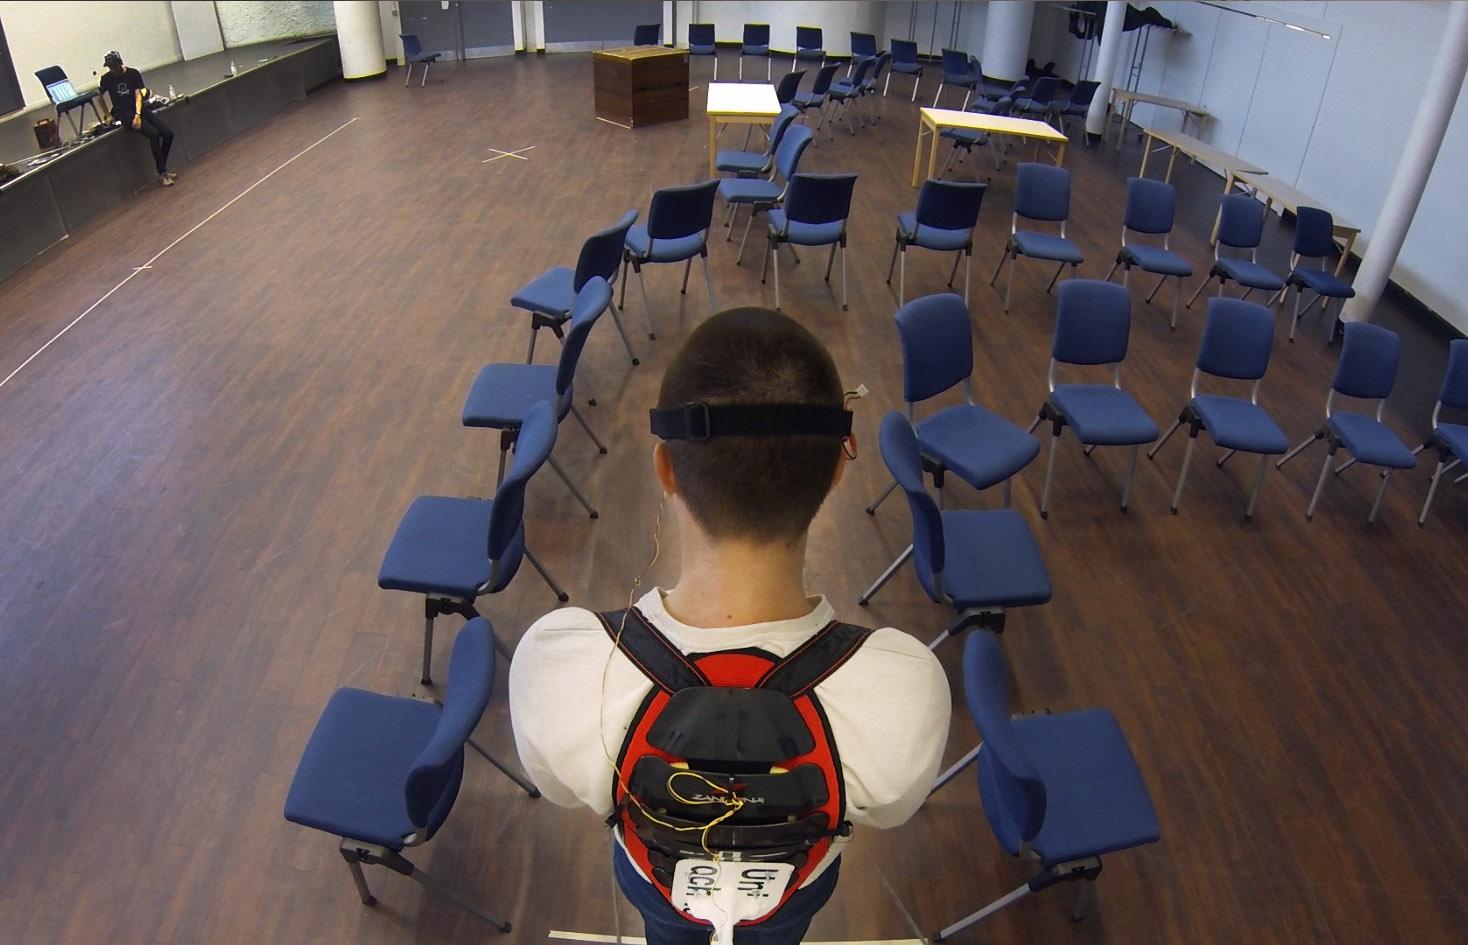
\includegraphics[width=\textwidth]{ExternalMaterial/3Pview}

   \caption{An approximate view of what the participant saw during the experiments. \label{fig:3Pview}}
\end{figure}



\begin{figure}
   \centering
   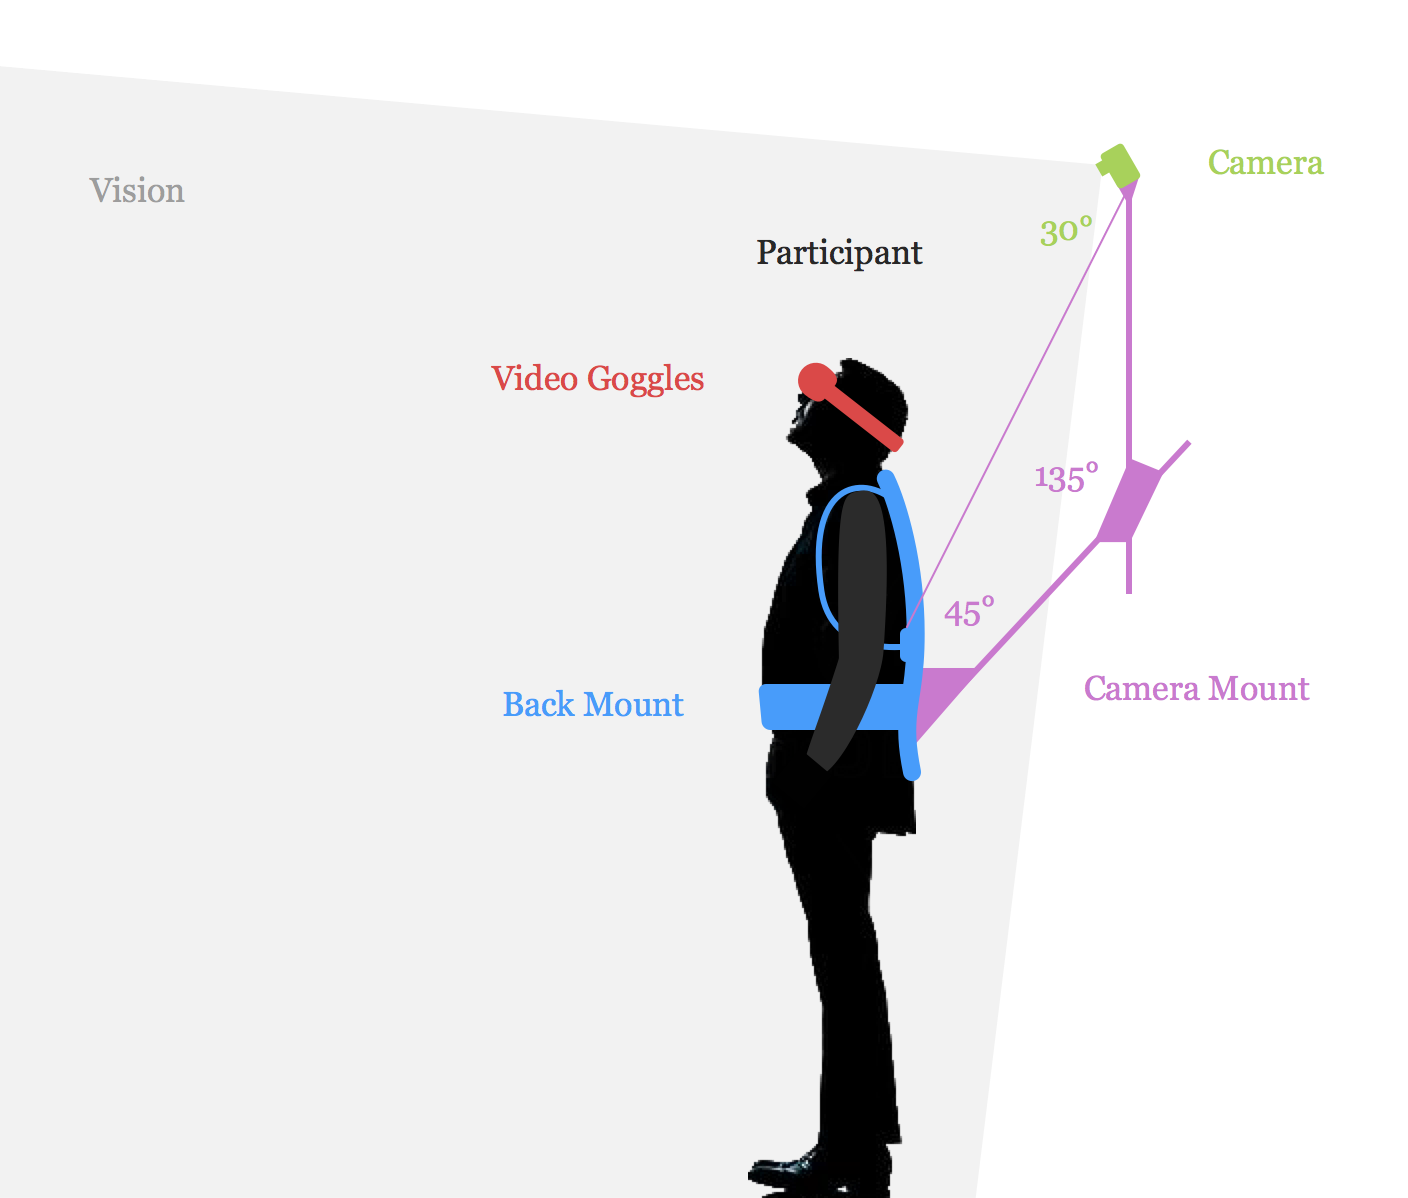
\includegraphics[width=\textwidth]{ExternalMaterial/Rig}
   \caption{A detailed overview of different parts of the rig. \label{fig:RigDesign}}
\end{figure}










\subsection{Survey Design}
After each test subject finished his/hers participation in the experiment they were prompted to fill out a survey (the full form can be found in the Appendix in Section~\ref{subsec:Survey})  regarding the experience during the experiment and their prior experience with video games. The survey included the following seven questions:
\begin{enumerate}
	\item Do you consider yourself a \emph{gamer}?
	\item What was the hardest parts in the experiment?
	\item On average, how many hours per week do you spend playing video games?
	\item How many years have you been playing video games?
	\item In total, how many hours have you spent playing a game viewed from a third-person perspective?
	\item If any, please name some of these third-person games you have played.
	\item Did you find your participation in this experiment fun?
\end{enumerate}
Each test subject also filled in details about their name, age and sex so the results from the test data could be paired up with the surveys. The details were later removed in the results in order to protect the test subjects anonymity.










% 8888888b.  8888888888 .d8888b.  888     888 888    88888888888 
% 888   Y88b 888       d88P  Y88b 888     888 888        888     
% 888    888 888       Y88b.      888     888 888        888     
% 888   d88P 8888888    "Y888b.   888     888 888        888     
% 8888888P"  888           "Y88b. 888     888 888        888     
% 888 T88b   888             "888 888     888 888        888     
% 888  T88b  888       Y88b  d88P Y88b. .d88P 888        888     
% 888   T88b 8888888888 "Y8888P"   "Y88888P"  88888888   888

\section{Results}
This section will cover the results from the tests that where done and;
\begin{itemize}
	\item The results from the tests - No significant findings
	\item Performance in the third-person perspective was generally worse than in first-person perspective.
	\item No difference between men and women
	\item Diagrams comparing the results
	\item Results of earlier work
	\item Compare the performance between the different groups
\end{itemize}

\subsection{Gamers versus Non-gamers}
Results when comparing the two groups, gamers and non-gamers.
\subsubsection{Accuracy Task}
This section will contain information about:
\begin{itemize}
	\item Gamers slightly better when wearing goggles, worse when not wearing goggles. No significant results unfortunately. See~\ref{fig:Task1GraphP}
	\item Differences between the first configuration and the other two were both lower for gamers than for non-gamers. Same for the differences between the second and third configuration. Gamers slightly performed \textbf{better}. See~\ref{fig:Task1GraphD}.
\end{itemize}

\begin{figure}
   \centering
   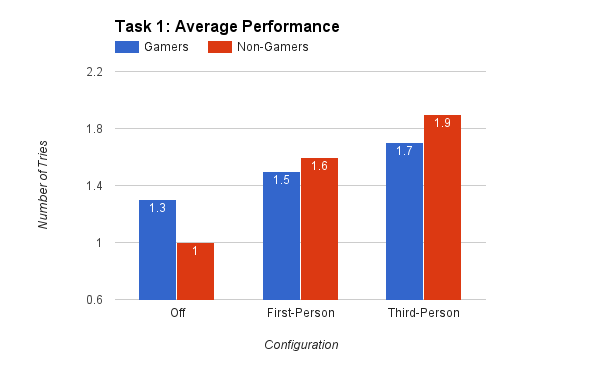
\includegraphics[width=\textwidth]{ExternalMaterial/Task1GraphP}
   \caption{Average performance (tries required, less is better) for the two groups for task 1.} \label{fig:Task1GraphP}
\end{figure}

\begin{figure}
   \centering
   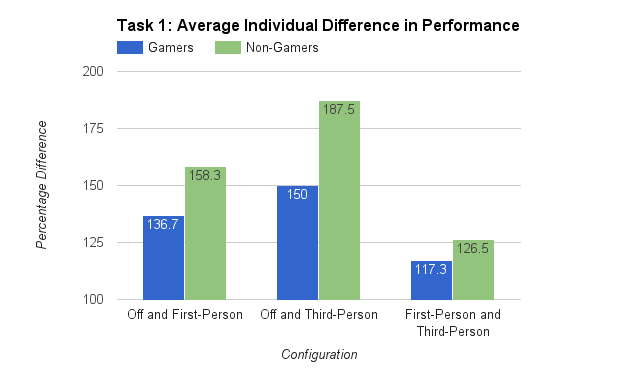
\includegraphics[width=\textwidth]{ExternalMaterial/Task1GraphD}
   \caption{Average individual difference (percent, less is better) in performance (tries required, less is better) between two configurations for the two groups for task 1.} \label{fig:Task1GraphD}
\end{figure}




\subsubsection{Balance Task}
This section will contain information about:
\begin{itemize}
	\item Gamers performed a little bit worse but no significant difference in the two later configurations. See~\ref{fig:Task2GraphP}
	\item Differences between the number of errors made in the first-person perspective (configuration 2) and the third-person perspective were larger for gamers than for non-gamers. Gamers performed slightly \textbf{worse}. See~\ref{fig:Task2GraphD}.
	%\item The results from this tests were generally bad due to the lack of vision of the line.
\end{itemize}

\begin{figure}
   \centering
   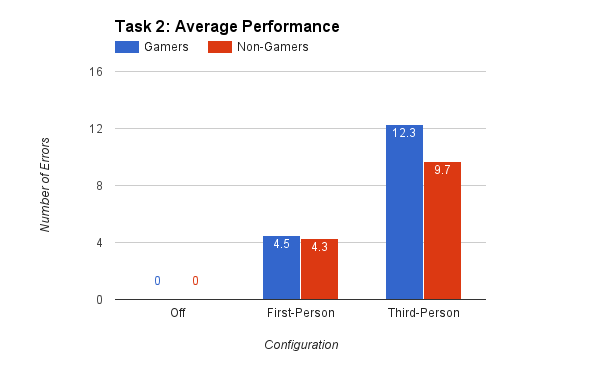
\includegraphics[width=\textwidth]{ExternalMaterial/Task2GraphP}
   \caption{Average performance (errors made, less is better) for the two groups for task 2.} \label{fig:Task2GraphP}
\end{figure}

\begin{figure}
   \centering
   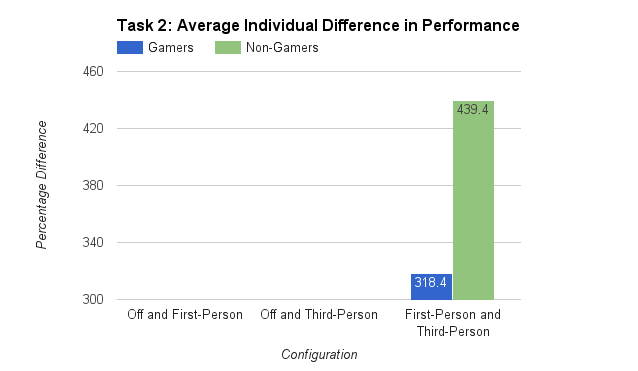
\includegraphics[width=\textwidth]{ExternalMaterial/Task2GraphD}
   \caption{Average individual difference (percent, less is better) in performance (errors made, less is better) between two configurations for the two groups for task 2.} \label{fig:Task2GraphD}
\end{figure}





\subsubsection{Movement Task}
This section will contain information about:
\begin{itemize}
	\item Gamers generally took longer time for all configurations. See~\ref{fig:Task3GraphP}
	\item Differences between the first configuration and the other two were both larger for gamers than for non-gamers. Same for the differences between the second and third configuration. Gamers slightly performed \textbf{worse}. See~\ref{fig:Task3GraphD}.
\end{itemize}

\begin{figure}
   \centering
   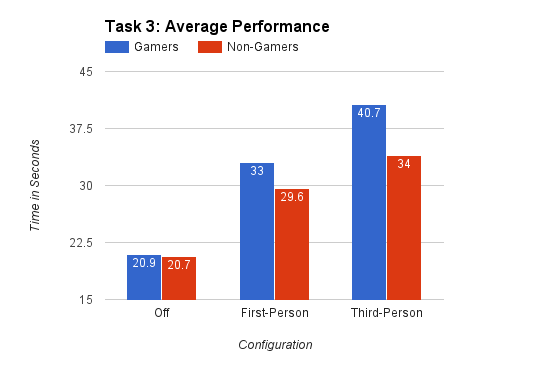
\includegraphics[width=\textwidth]{ExternalMaterial/Task3GraphP}
   \caption{Average performance (time required, less is better) for the two groups for task 3.} \label{fig:Task3GraphP}
\end{figure}

\begin{figure}
   \centering
   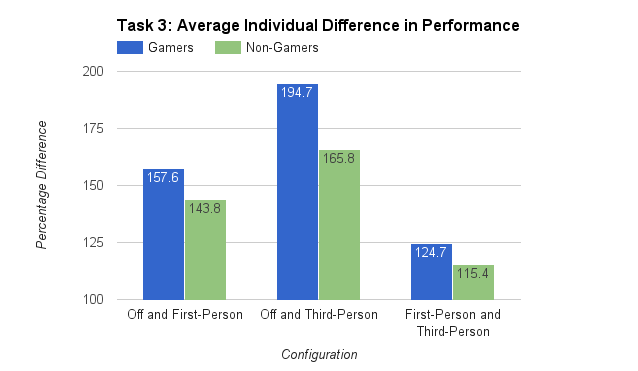
\includegraphics[width=\textwidth]{ExternalMaterial/Task3GraphD}
   \caption{Average individual difference (percent, less is better) in performance (time required, less is better) between two configurations for the two groups for task 3.} \label{fig:Task3GraphD}
\end{figure}










% 8888888b. 8888888 .d8888b.   .d8888b.  888     888  .d8888b.   .d8888b.  
% 888  "Y88b  888  d88P  Y88b d88P  Y88b 888     888 d88P  Y88b d88P  Y88b 
% 888    888  888  Y88b.      888    888 888     888 Y88b.      Y88b.      
% 888    888  888   "Y888b.   888        888     888  "Y888b.    "Y888b.   
% 888    888  888      "Y88b. 888        888     888     "Y88b.     "Y88b. 
% 888    888  888        "888 888    888 888     888       "888       "888 
% 888  .d88P  888  Y88b  d88P Y88b  d88P Y88b. .d88P Y88b  d88P Y88b  d88P 
% 8888888P" 8888888 "Y8888P"   "Y8888P"   "Y88888P"   "Y8888P"   "Y8888P"  

\section{Discussion}
A general discussion about the study such as:
\begin{itemize}
	\item What part/conclusion in my study could be biast/not reliable
	\item What does my results mean?
	\item Earlier work, how do they compare to my work and what does that mean?
	\item References to earlier work such as~\cite{schmierbach2011exploring}
	\item What defines a gamer? How many hours played etc.
\end{itemize}



\subsection{Limitations and Drawbacks}
Due to the time and budget limit there are several ways to improve upon my study, ways of doing this might include:
\begin{description}
	\item[Rig Design] Building a more rigid rig.
	\item[Task Design] Using a more comprehensive camera mounted on a stabilized gimbal.
	\item[Video Goggles] Using more sophisticated video goggles, such as the Oculus Rift.
	\item[More Segregated Groups] Gamers and non-gamers
	\item[Sex Ratio] Hard finding gamer women.
\end{description}




\subsection{Conclusion}
As a finish, and a complement to the abstract, the conclusion should contain:
\begin{itemize}
	\item What to take out from the study
	\item How this study can be made more in-depth
	\item Future work
\end{itemize}











%        d8888  .d8888b.  888    d8P  888b    888  .d88888b.  888       888 
%       d88888 d88P  Y88b 888   d8P   8888b   888 d88P" "Y88b 888   o   888 
%      d88P888 888    888 888  d8P    88888b  888 888     888 888  d8b  888 
%     d88P 888 888        888d88K     888Y88b 888 888     888 888 d888b 888 
%    d88P  888 888        8888888b    888 Y88b888 888     888 888d88888b888 
%   d88P   888 888    888 888  Y88b   888  Y88888 888     888 88888P Y88888 
%  d8888888888 Y88b  d88P 888   Y88b  888   Y8888 Y88b. .d88P 8888P   Y8888 
% d88P     888  "Y8888P"  888    Y88b 888    Y888  "Y88888P"  888P     Y888 

\section{Acknowledgments}
The authors would like to thank all participants in the study for their time, participation and feedback. We would also like to thank all the peer-reviewers (especially \emph{Lars Englund} for his unquestionable loyalty and help during the experiments) who helped form this report into its final shape. Last but not least we would like to thank \emph{Umeå University} for letting us use their facilities \emph{Rotundan} (where we conducted our experiments) and \emph{Robot Labbet} (where we built the rig) during the progress of the report.







%\nocite{*}
\bibliographystyle{splncs}
%\bibliographystyle{plain-annote}

\bibliography{Bibliography}

\appendix

\section{Appendix}
All the files for this report, along with all the 3D-design-files can be found and downloaded on the GitHub page for this project: https://github.com/Kodagrux/Third-Person-Performance-Differences-Between-Gamers-and-Nongamers 
\subsection{Survey} \label{subsec:Survey}
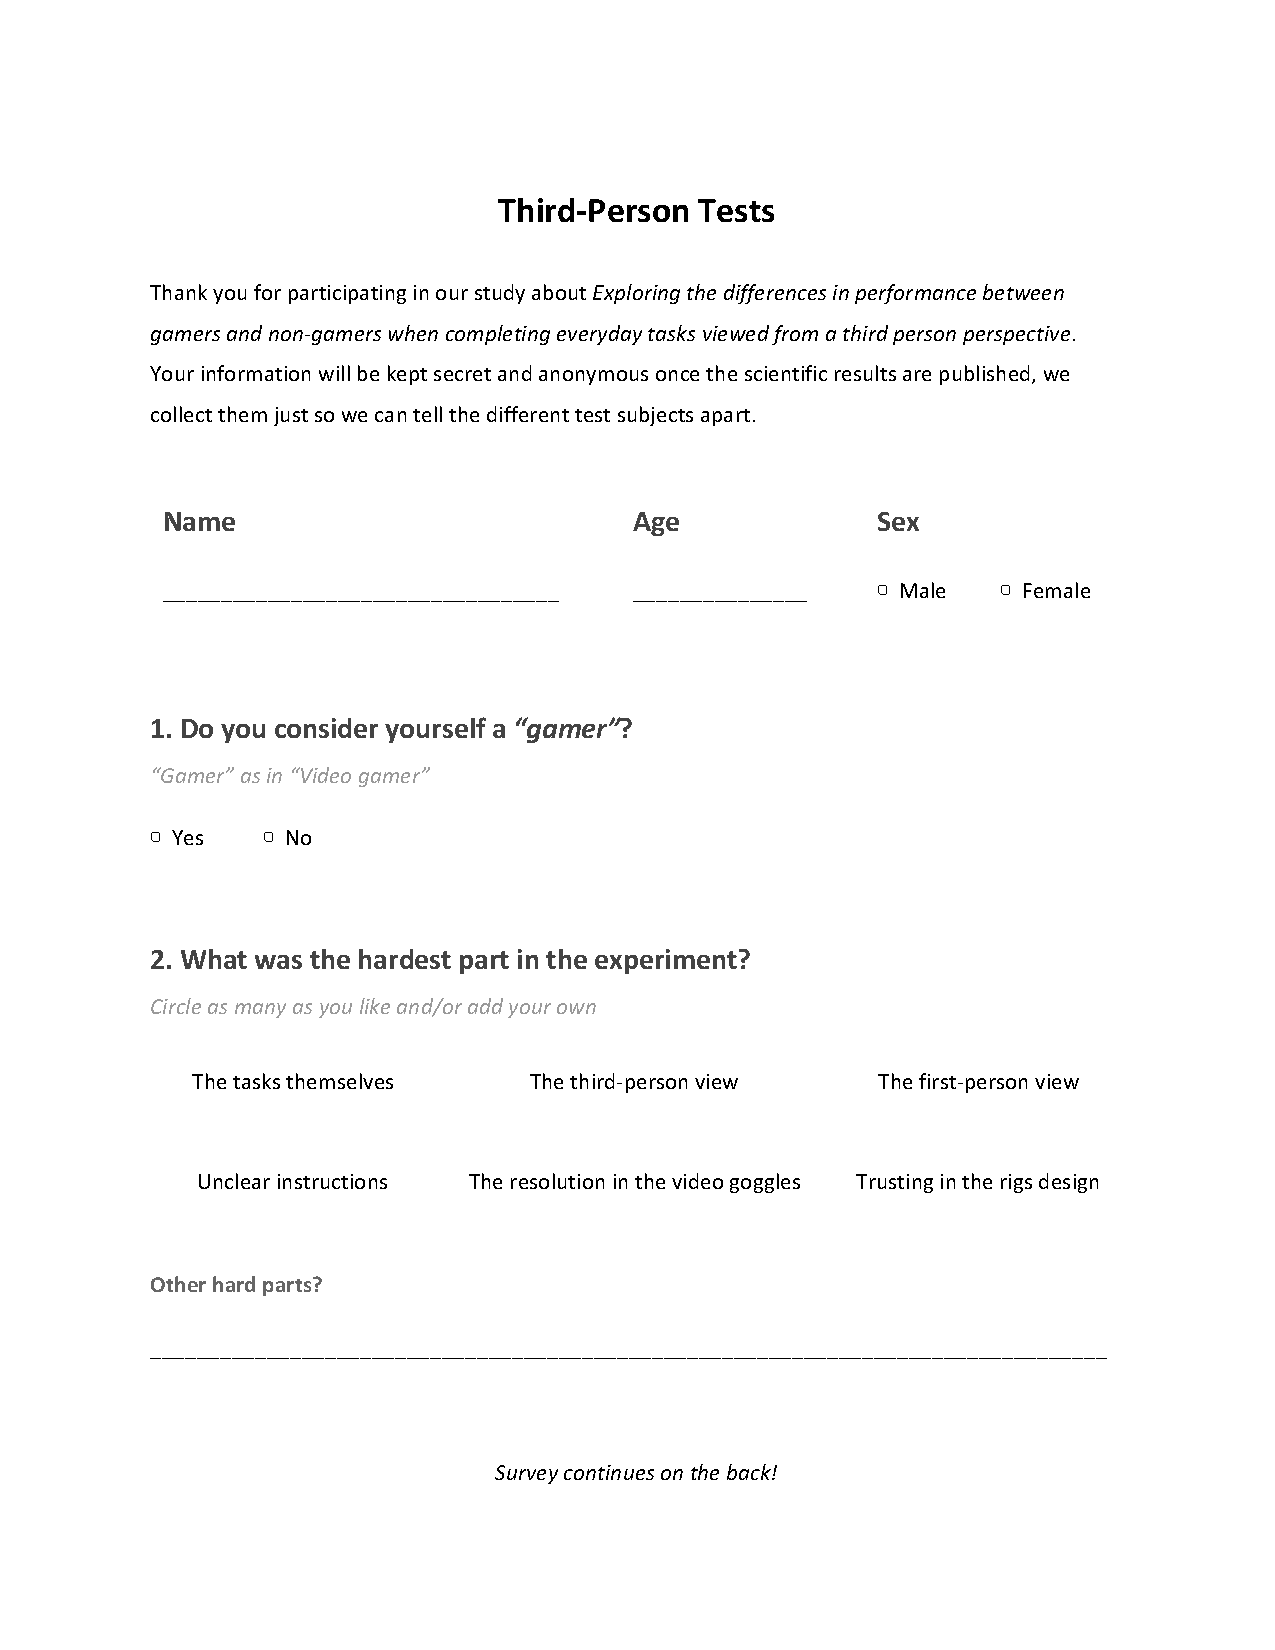
\includepdf[pages={1-2}]{ExternalMaterial/Survey.pdf}


\end{document}